\chapter{Implementasi dan Pengujian Aplikasi}
\label{chap:Implementasi dan Pengujian Aplikasi}

Pada bab 5 dibahas implementasi dan pengujian aplikasi Pencari Rute Kendaraan Umum untuk Windows Phone.

%Implementasi
\section{Implementasi}
\label{lab:Implementasi}
\hspace{0.5cm} Pada sub-bab ini dijelaskan mengenai lingkungan yang digunakan untuk membangun aplikasi Pencari Rute Kendaraan Umum untuk Windows Phone dan hasil dari implementasi. Lingkungan implementasi yang dibahas meliputi perangkat lunak untuk implementasi dan perangkat keras untuk implementasi. Hasil dari implementasi juga disampaikan dalam bentuk \textit{screenshoot} ketika aplikasi dijalankan.

%Perangkat Keras untuk Implementasi
\subsection{Perangkat Keras untuk Implementasi}
\label{lab:Perangkat Keras untuk Implementasi}
\hspace{0.5cm} Dalam membangun aplikasi ini perangkat keras yang digunakan adalah sebagai berikut:
\begin{enumerate}
	\item Komputer
		\begin{enumerate}
			\item \textit{Processor}: intel Core i7-2620M CPU 2,7 GHz
			\item RAM: 4 GB
			\item \textit{Hardisk}: 640 GB
			\item VGA: Intel HD 3000
		\end{enumerate}
		
	\item Perangkat \textit{Mobile}
		\begin{enumerate}
			\item \textit{Processor}: 1,2 GHz
			\item RAM: 1 GB
			\item ROM: 8 GB
			\item Layar: 720 x 1280 pixel, 4,7 inch
			\item GPS
			\item Sensor: kompas, \textit{accelerometer}
		\end{enumerate}
\end{enumerate}

%Perangkat Lunak untuk Implementasi
\subsection{Perangkat Lunak untuk Implementasi}
\label{lab:Perangkat Lunak untuk Implementasi}
\hspace{0.5cm} Dalam membangun aplikasi ini perangkat lunak yang digunakan adalah sebagai berikut:
\begin{enumerate}
	\item Komputer
		\begin{enumerate}
			\item Sistem Operasi Windows 8.1
			\item IDE Visual Studio Express 2012
			\item Bahasa Pemrograman C\#
			\item Library .Net Framework 4.5
		\end{enumerate}
		
	\item Perangkat \textit{mobile}
		\begin{enumerate}
			\item Sistem Operasi Windows Phone 8.1
		\end{enumerate}
\end{enumerate}

%Hasil Implementasi
\subsection{Hasil Implementasi}
\label{lab:Hasil Implementasi}
\hspace{0.5cm} Hasil implementasi dari perangkat lunak ini terbagi dalam tiga bagian, yaitu:
\begin{enumerate}
	\item Kode program \\
	Kode Program pada perangkat lunak ditulis dengan menggunakan bahasa C\#. Bahasa C\# dipilih berdasarkan analisa pada bab 3.
	\item Hasil kompilasi program \\
	Hasil dari kompilasi program berupa \textit{file} Kiri\_Debug\_AnyCPU.xap. \textit{File} ini dapat dipasang pada perangkat dengan sistem operasi Windows Phone versi 8 atau lebih tinggi.
	\item Antarmuka aplikasi \\
	Berikut merupakan hasil implementasi antarmuka aplikasi Pencari Rute Kendaraan Umum untuk Windows phone.
\end{enumerate}

% Gambar antarmuka kelas MainPage
	\begin{figure}[!h]
		\centering
			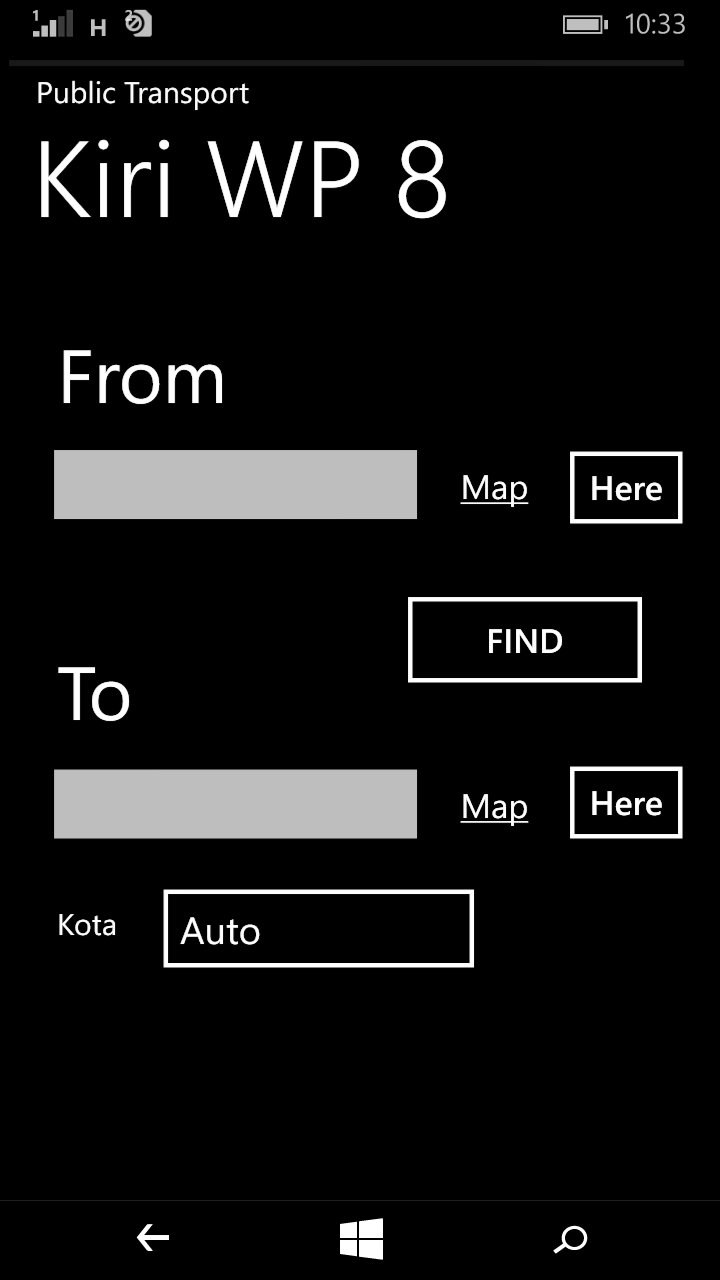
\includegraphics[scale=0.25]{Gambar/antarmuka/home}
		\caption{Gambar antarmuka kelas MainPage}
		\label{fig:antarmuka MainPage}
	\end{figure}
	
	\newpage
	
	% Gambar antarmuka Splash MainPage
	\begin{figure}[!h]
		\centering
			
\includegraphics[scale=0.22]{Gambar/antarmuka/splash}
		\caption{Gambar Antarmuka Splash di Kelas MainPage}
		\label{fig:antarmuka splash MainPage}
	\end{figure}	
	
	% Gambar antarmuka list di kelas MainPage
	\begin{figure}[!h]
		\centering
			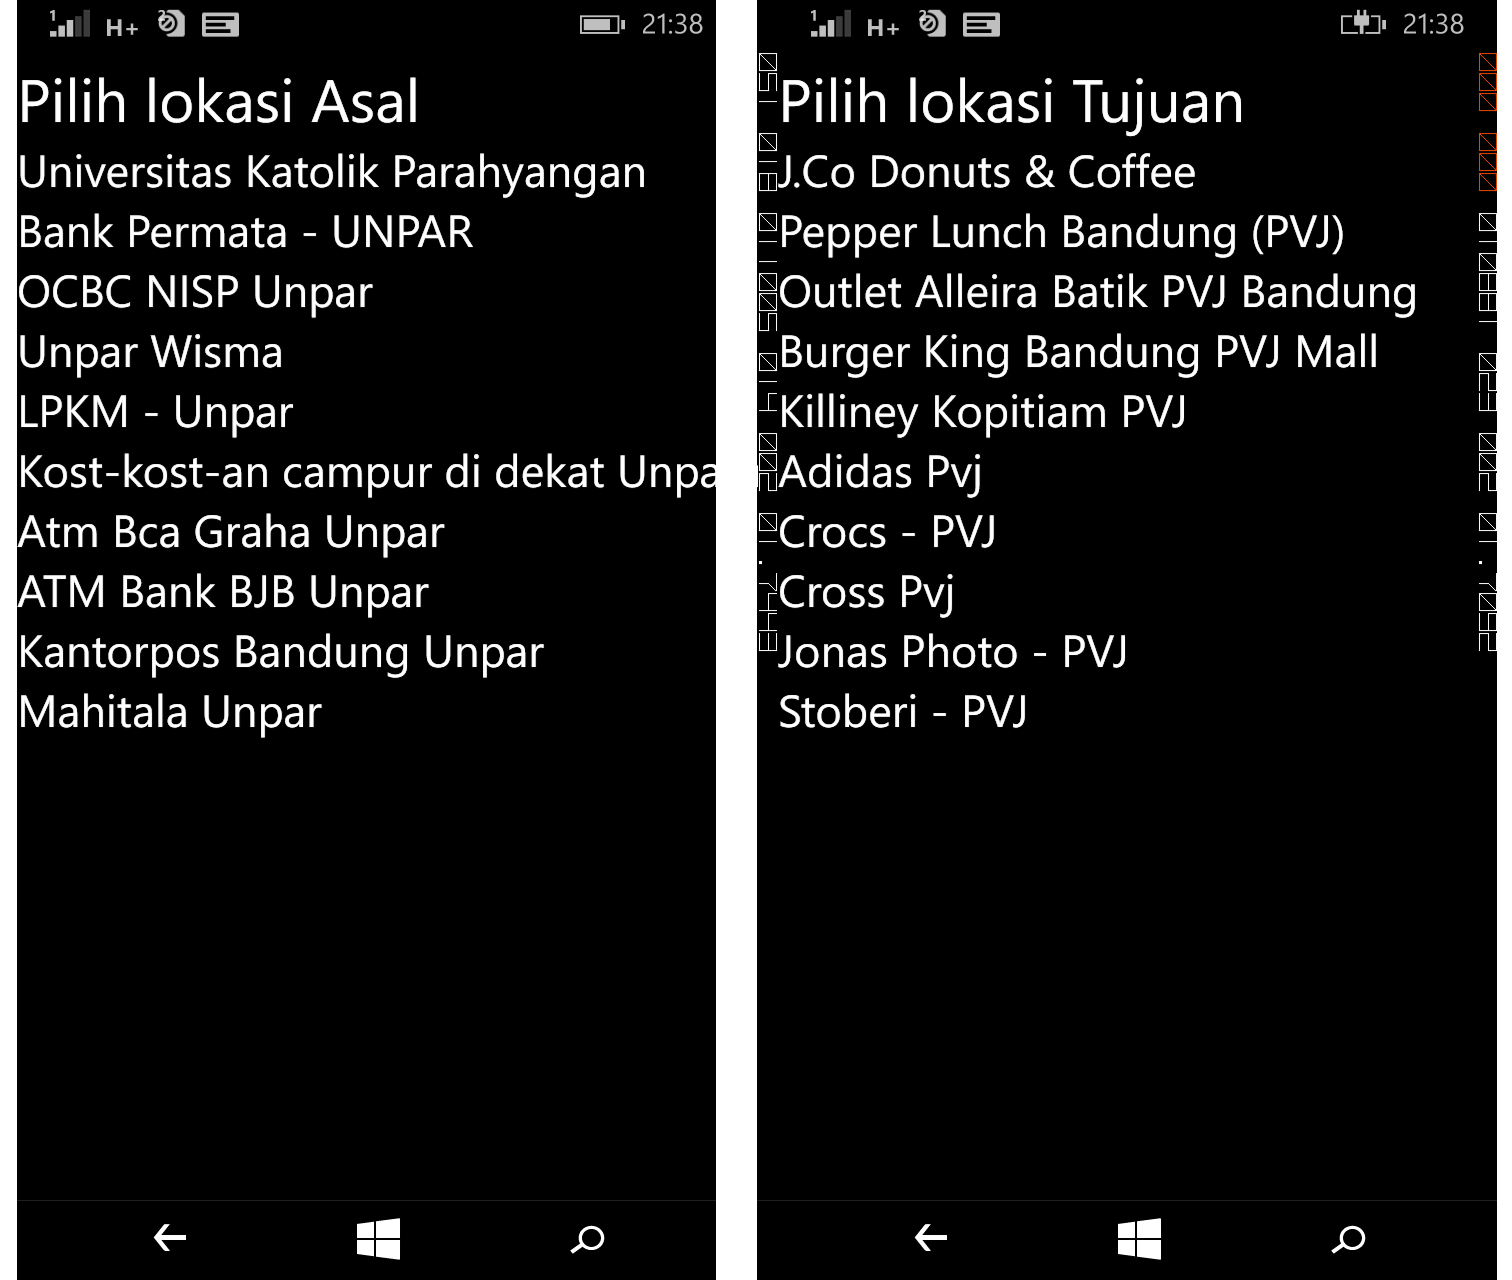
\includegraphics[scale=0.22]{Gambar/antarmuka/list_main}
		\caption{Gambar Antarmuka \textit{List} Asal dan \textit{List} Tujuan di Kelas MainPage}
		\label{fig:antarmuka list MainPage}
	\end{figure}
	
	\newpage
	% Gambar antarmuka kelas Map
	\begin{figure}[!h]
		\centering
			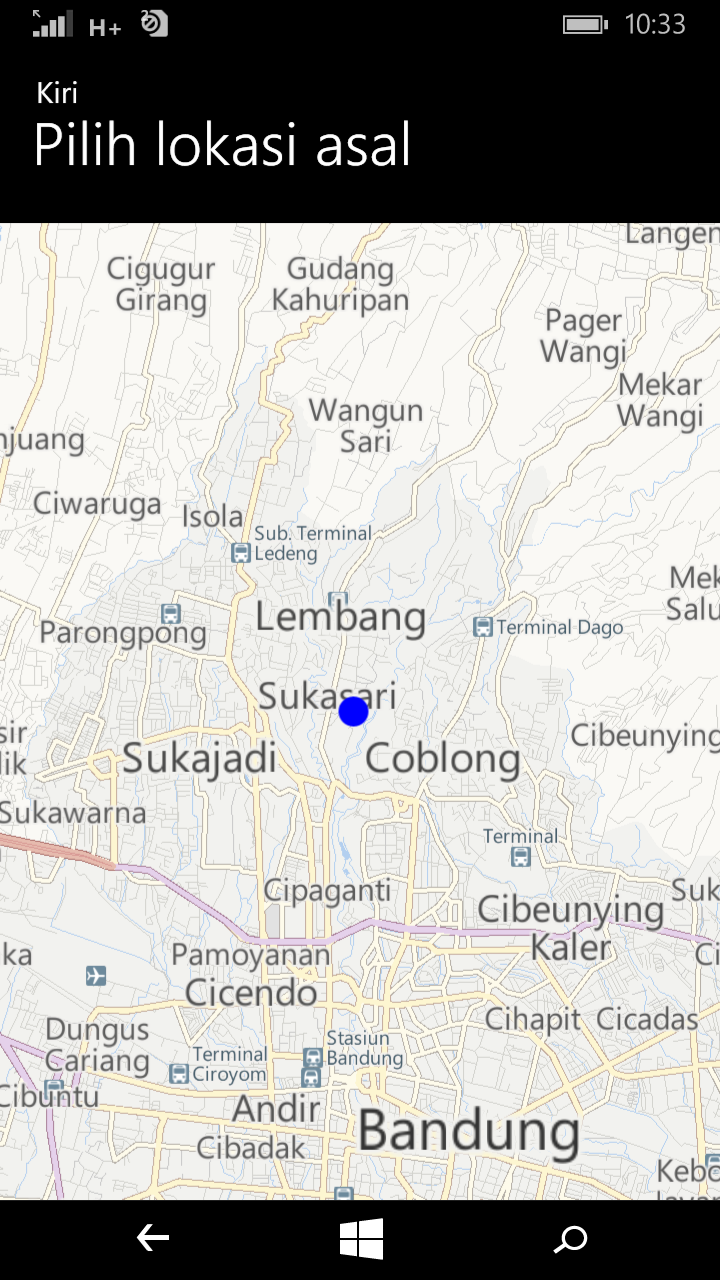
\includegraphics[scale=0.22]{Gambar/antarmuka/map}
		\caption{Gambar Antarmuka Kelas Map}
		\label{fig:antarmuka Map}
	\end{figure}
	
	% Gambar antarmuka menunggu di kelas Route
	\begin{figure}[!h]
		\centering
			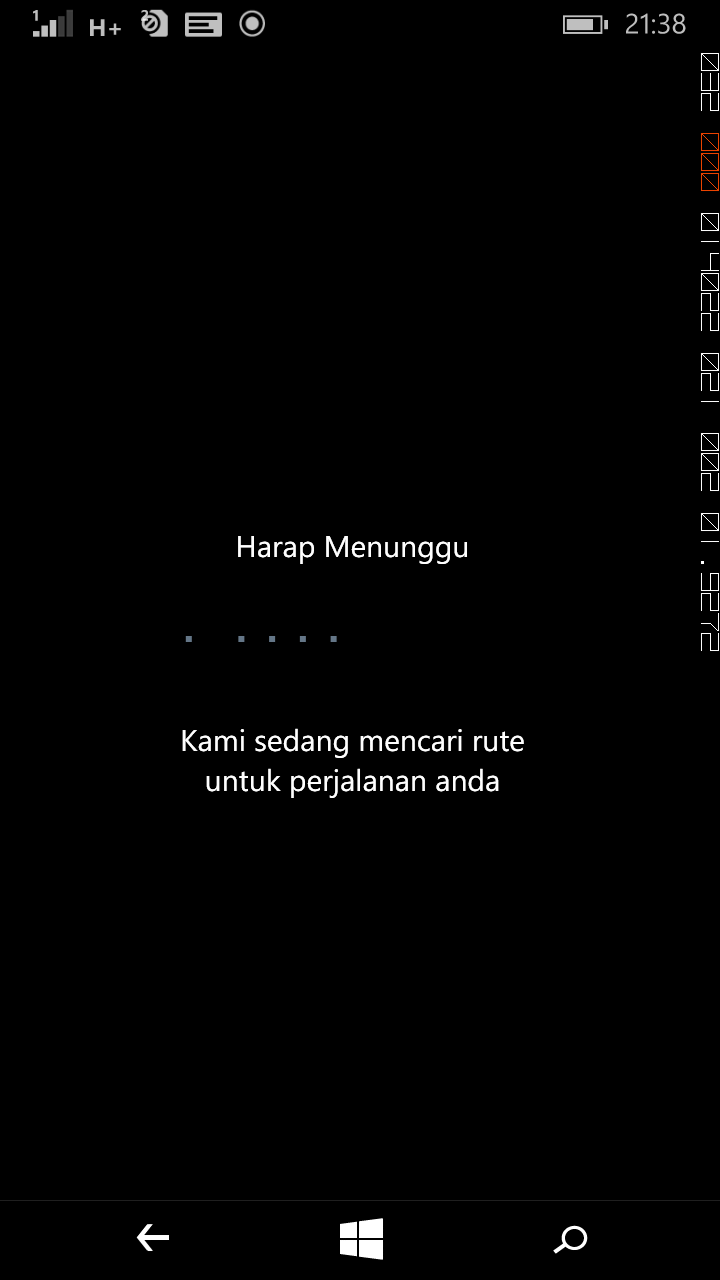
\includegraphics[scale=0.22]{Gambar/antarmuka/wait_route}
		\caption{Gambar Antarmuka Menunggu di Kelas Route}
		\label{fig:antarmuka menunggu Route}
	\end{figure}
	
	% Gambar antarmuka kelas Route
	\begin{figure}[!h]
		\centering
			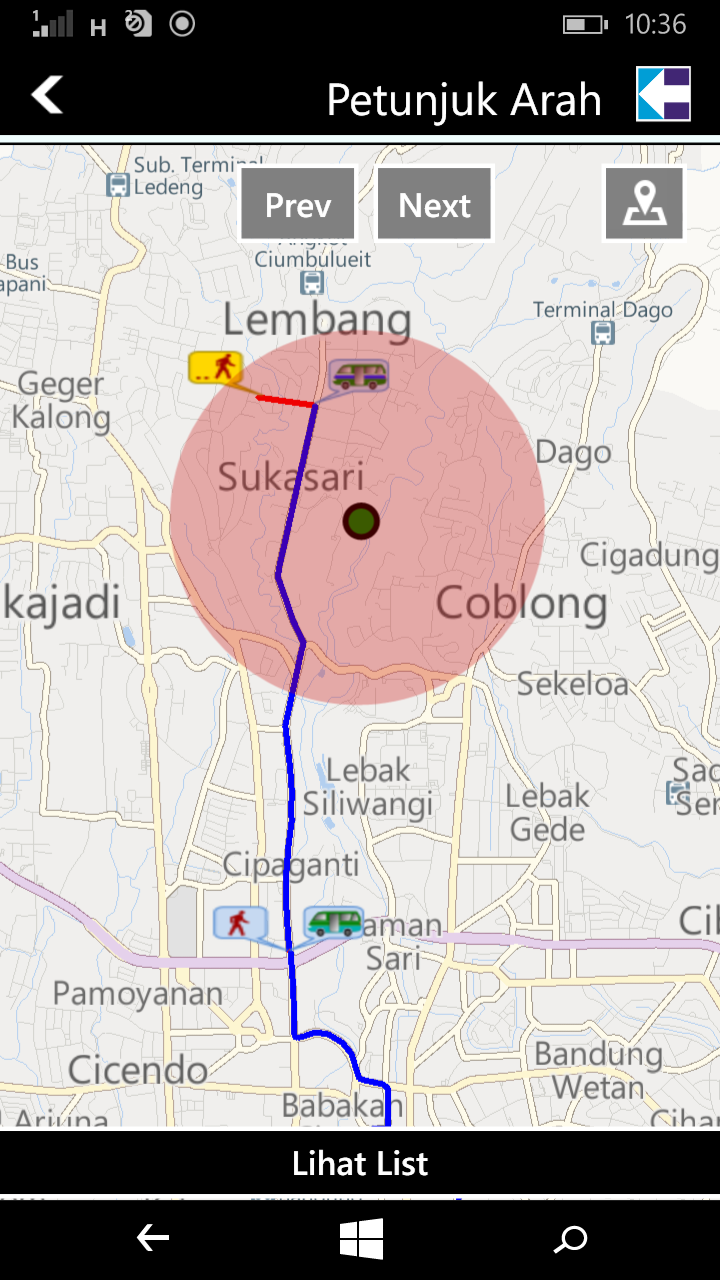
\includegraphics[scale=0.22]{Gambar/antarmuka/route_map}
		\caption{Gambar Antarmuka Kelas Route}
		\label{fig:antarmuka Route}
	\end{figure}
	
	\newpage
	% Gambar antarmuka kelas Route bentuk list
	\begin{figure}[!h]
		\centering
			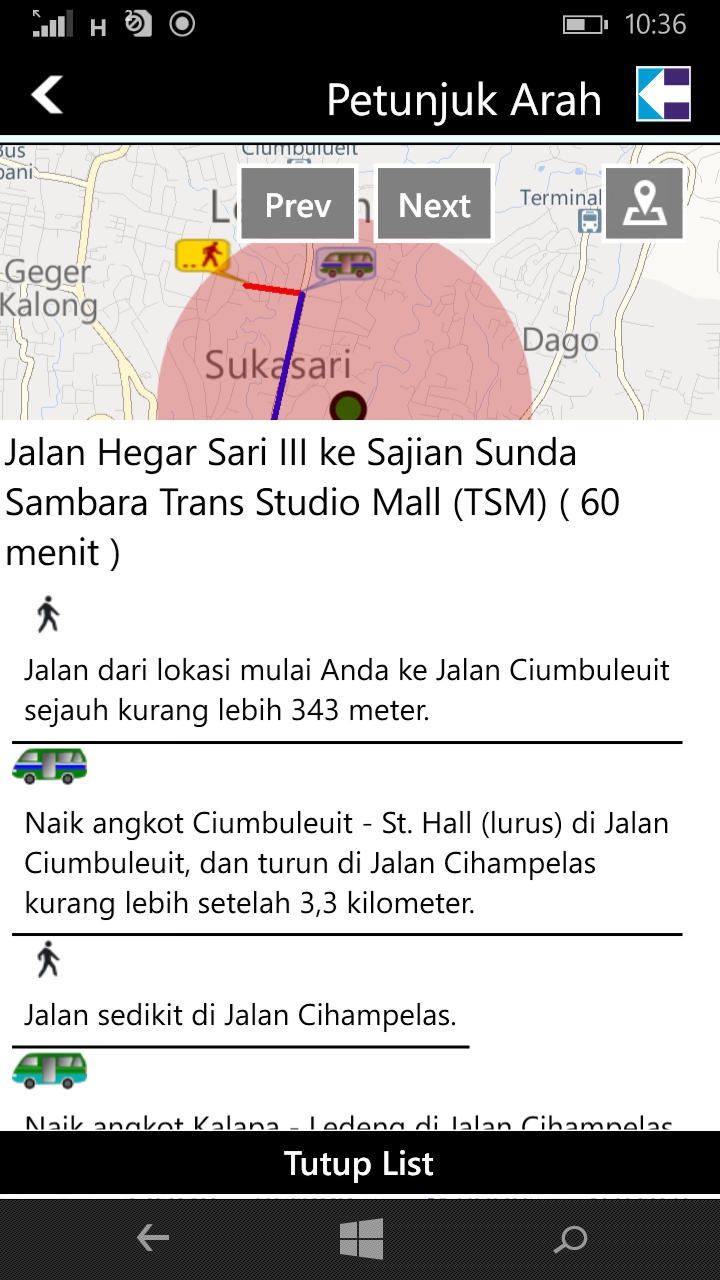
\includegraphics[scale=0.25]{Gambar/antarmuka/list_route}
		\caption{Gambar Antarmuka \textit{List} di Kelas Route}
		\label{fig:antarmuka list Route}
	\end{figure}

\newpage

%Pengujian
\section{Pengujian}
\label{lab:Pengujian}
\hspace{0.5cm} Pada bagian ini dibahas mengenai hasil pengujian yang telah dilakukan terhadap aplikasi yang telah dibangun. Pengujian yang dilakukan terdiri dari dua bagian yaitu pengujian fungsional dan pengujian eksperimental. Pengujian fungsional bertujuan untuk memastikan semua fungsi aplikasi berjalan sesuai harapan. Sementara pengujian eksperimental bertujuan untuk mengetahui keberhasilan proses kerja dari aplikasi.

%Lingkungan Pengujian
\subsection{Lingkungan Pengujian}
\label{lab:Lingkungan Pengujian}
\hspace{0.5cm} Dalam proses pengujian perangkat lunak digunakan sistem operasi Windows Phone 8.1 dengan spesifikasi perangkat keras sebagai berikut.
\begin{enumerate}
	\item \textit{Processor} : 1.2 Ghz Quad Core
	\item RAM : 1 GB
	\item Layar : 1280 x 720 \textit{pixels}, 4,7 inch
	\item GPS : A-GPS, GLONASS, Beidou
\end{enumerate}

%Pengujian Fungsional untuk mengetahui kesesuaian reaksi nyata dengan yang diharapkan
\subsection{Pengujian Fungsional}
\label{lab:Pengujian Fungsional}
\hspace{0.5cm} Pengujian fungsional dilakukan untuk menguji kesesuaian reaksi yang terjadi dengan reaksi yang diharapkan. Untuk menguji kesesuaian reaksi yang terjadi dengan reaksi yang diharapkan penulis menguji 5 orang pengguna. Pengujian ini hanya sebatas pencarian rute dengan area terbatas di satu kota yaitu Bandung. Kelima pengguna tersebut terdiri dari 3 orang mahasiswa dari luar Bandung yang kuliah di Unpar dan 2 orang mahasiswa asli Bandung yang kuliah di Unpar. Kelima pengguna tersebut semuanya pernah menggunakan transportasi umum terutama angkutan kota. Kelima pengguna tersebut dipinjamkan perangkat untuk mencari rute dengan perintah sebagai berikut. 
\begin{enumerate}
	\item Carilah rute dari sini ke BIP!
	\item Carilah rute dari BIP ke Ciwalk!
	\item Carilah rute dari sini ke ITB pintu jalan Ganesa!
\end{enumerate}

Dari tiga perintah berikut, penulis mengharapkan hasil sebagi berikut.
\begin{table}[h]
	\centering
		\begin{tabular}{|p{2cm}|p{10cm}|}\hline
				Perintah & Aksi Pengguna \\ \hline
				1 & Mencari lokasi dengan tombol "Here" dan menulis kata "bip" pada \textit{textbox} \\ \hline
				2 & Menulis kata "bip" pada \textit{textbox} dan menulis kata "Ciwalk" pada \textit{textbox} \\ \hline
				3 & Mencari lokasi dengan tombol "Here" dan menunjuk pintu masuk ITB yang di jalan Ganesa \\ \hline
		\end{tabular}
	\caption{Tabel Hasil yang Diharapkan Penulis untuk Pengujian}
	\label{tab:TabelHasilyangdiharapkanPenulis}
\end{table}

Dari tiga perintah berikut didapat hasil sebagi berikut.
\begin{table}[h!]
	\centering
		\begin{tabular}{|p{1,5cm}|p{9cm}|p{2cm}|}\hline
				Perintah & Aksi Pengguna & Kesesuaian \\ \hline
				1 & Mencari lokasi dengan tombol "Here" dan menulis "BIP" pada \textit{textbox} & sesuai \\ \hline
				2 & Menulis "BIP" pada \textit{textbox} dan menulis "Ciwalk" pada \textit{textbox} & sesuai \\ \hline
				3 & Mencari lokasi dengan tombol "Here" dan menulis "jl Ganesa" pada \textit{textbox} & tidak sesuai \\ \hline
		\end{tabular}
	\caption{Tabel Hasil Pengujian Fungsionalitas Terhadap Pengguna 1}
	\label{tab:TabelHasilPengujianFungsionalitasTerhadapPengguna}
\end{table}

\begin{table}[h!]
	\centering
		\begin{tabular}{|p{1,5cm}|p{9cm}|p{2cm}|}\hline
				Perintah & Aksi Pengguna & Kesesuaian \\ \hline
				1 & Mencari lokasi dengan tombol "Here" dan menulis "BIP" pada \textit{textbox} & sesuai \\ \hline
				2 & Menulis "BIP" pada \textit{textbox} dan menulis "Ciwalk" pada \textit{bextbox} & sesuai \\ \hline
				3 & Mencari lokasi dengan tombol "Here" dan menunjuk pada peta & sesuai \\ \hline
		\end{tabular}
	\caption{Tabel Hasil Pengujian Fungsionalitas Terhadap Pengguna 2}
	\label{tab:TabelHasilPengujianFungsionalitasTerhadapPengguna}
\end{table}

\begin{table}[h!]
	\centering
		\begin{tabular}{|p{1,5cm}|p{9cm}|p{2cm}|}\hline
				Perintah & Aksi Pengguna & Kesesuaian \\ \hline
				1 & Mencari lokasi dengan tombol "Here" dan menulis "BIP" pada \textit{textbox} & sesuai \\ \hline
				2 & Menulis "BIP" pada \textit{textbox} dan menulis "CIwalk" pada \textit{textbox} & sesuai \\ \hline
				3 & Mencari lokasi dengan tombol "Here" dan menulis "ITB Ganeca" pada TextBox lalu menyadari tombol map dan menggunakannya & sesuai \\ \hline
		\end{tabular}
	\caption{Tabel Hasil Pengujian Fungsionalitas Terhadap Pengguna 3}
	\label{tab:TabelHasilPengujianFungsionalitasTerhadapPengguna}
\end{table}

\newpage

\begin{table}[h!]
	\centering
		\begin{tabular}{|p{1,5cm}|p{9cm}|p{2cm}|}\hline
				Perintah & Aksi Pengguna & Kesesuaian \\ \hline
				1 & Mencari lokasi dengan tombol "Here" dan menulis "BIP" pada \textit{textbox} & sesuai \\ \hline
				2 & Menulis "BIP" pada \textit{textbox} dan menulis "Ciwalk" pada \textit{textbox} & sesuai \\ \hline
				3 & Mencari lokasi dengan tombol "Here" dan menulis "Institut Teknologi Bandung" pada \textit{textbox} & tidak sesuai \\ \hline
		\end{tabular}
	\caption{Tabel Hasil Pengujian Fungsionalitas Terhadap Pengguna 4}
	\label{tab:TabelHasilPengujianFungsionalitasTerhadapPengguna}
\end{table}

\begin{table}[h!]
	\centering
		\begin{tabular}{|p{1,5cm}|p{9cm}|p{2cm}|}\hline
				Perintah & Aksi Pengguna & Kesesuaian \\ \hline
				1 & Mencari lokasi dengan tombol "Here" dan menulis "BIP" pada \textit{textbox} & sesuai \\ \hline
				2 & Menulis "BIP" pada \textit{textbox} dan menulis "Ciwalk" pada \textit{textbox} & sesuai \\ \hline
				3 & Mencari lokasi dengan tombol "Here" dan menulis "jalan ganesa" pada \textit{textbox} & tidak sesuai \\ \hline
		\end{tabular}
	\caption{Tabel Hasil Pengujian Fungsionalitas Terhadap Pengguna 5}
	\label{tab:TabelHasilPengujianFungsionalitasTerhadapPengguna}
\end{table}

\hspace{0.5cm} Hasil pengujian menunjukan untuk perintah 1 dan 2 semua pengguna dapat menyelesaikan perintah dengan aksi yang sesuai. Sedangkan untuk perintah ke 3 sebagian pengguna masih salah dalam melakukan aksi yang sesuai. Dari hasil pengujian terhadap pengguna dapat dilihat pengguna lebih memilih untuk mengetikan kata kunci karena hal tersebut adalah yang paling mudah untuk dilakukan. Pengguna cenderung memikirkan suatu lokasi, memikirkan kata kunci lalu menuliskannya pada textbox di aplikasi. Menuliskan pada \textit{textbox} memang lebih mudah dilakukan tapi ada beberapa pencarian spesifik yang tidak dapat dilakukan dengan mengetikan kata kunci.   

%start comment
\iffalse
Pengujian fungsionalitas digunakan untuk menguji aksi dan reaksi dari aplikasi. Hasil pengujian tersebut ditunjukan pada tabel ~\ref{tab:TabelHasilPengujianFungsionalitas}.
\begin{table}[h!]
	\centering
		\begin{tabular}{|p{1cm}|p{4cm}|p{6cm}|p{3cm}|}\hline
				No & Aksi Pengguna & Reaksi yang Diharapkan & Reaksi Perangkat lunak \\ \hline
				1 & Menjalankan aplikasi & Aplikasi menampilkan SplashScreen selama beberapa saat dan tampilan awal halaman MainPage ditampilkan & sesuai \\ \hline
				2 & Memasukan lokasi asal dan lokasi tujuan dari \textit{textbox} & \textit{Textbox} terisi sesuai masukan & sesuai \\ \hline
				3 & Memasukan lokasi asal atau lokasi tujuan berdasarkan lokasi perangkat dengan menekan tombol "here" & \textit{Textbox} lokasi asal atau lokasi tujuan terisi "here" & sesuai \\ \hline
				4 & Menekan tombol "maps" untuk memilih lokasi pada peta & Pindah halaman ke kelas Map & sesuai \\ \hline
				5 & Menekan lokasi pada peta lalu menekan tombol "pilih lokasi" & Lokasi ditandai dan pengguna diarahkan kembali ke kelas Main Page & sesuai \\ \hline
				6 & Memilih kota & Kota berubah sesusai yang dipilih pengguna & sesuai \\ \hline
				7 & Menekan tombol "Find" & Bila lokasi diambil dari peta dan lokasi perangkat maka tidak akan tampil \textit{ListBox} dan antarmuka dialihkan ke kelas Route & sesuai \\ \hline
				8 & & Bila input masukan berupa kata kunci tempat maka akan tampil \textit{ListBox} untuk dipilih, lalu setelah dipilih antarmuka dialihkan ke kelas Route & sesuai \\ \hline
				9 & Bila \textit{ListBox} ditampilkan dan pengguna memilih & \textit{ListBox} akan tertutup & sesuai \\ \hline
				10 & Pada kelas Route pengguna menekan tombol "here" & Pusat peta akan diarahkan ke lokasi pengguna berada & sesuai \\ \hline
				11 & Pada kelas Route pengguna menekan tombol "Tunjukan Daftar" & Jika daftar tertutup maka daftar akan terbuka & sesuai \\ \hline
				12 & & Jika daftar terbuka maka daftar akan tertutup & sesuai \\ \hline
				13 & Pada kelas Route pengguna menekan tombol "Next" & Pusat peta akan diarahkan ke pergantian transportasi berikutnya sesua kembalian Kiri disertai keterangan & sesuai \\ \hline
		\end{tabular}
	\caption{Tabel Hasil Pengujian Fungsionalitas}
	\label{tab:TabelHasilPengujianFungsionalitas}
\end{table}

\begin{table}[h!]
	\centering
		\begin{tabular}{|p{1cm}|p{4cm}|p{6cm}|p{3cm}|}\hline
				No & Aksi Pengguna & Reaksi yang Diharapkan & Reaksi Perangkat lunak \\ \hline
				14 & Pada kelas Route pengguna menekan tombol "Prev" & Pusat peta akan diarahkan ke pergantian transportasi sebelumnya sesua kembalian Kiri disertai keterangan & sesuai \\ \hline
				15 & Pada kelas Route pengguna menekan tombol "windows" & Keadaan aplikasi menjadi \textit{dormant} & tidak sesuai \\ \hline
		\end{tabular}
	\caption{Tabel Hasil Pengujian Fungsionalitas}
	\label{tab:TabelHasilPengujianFungsionalitas}
\end{table}
\fi
%end comment

%https://msdn.microsoft.com/en-us/library/windows/apps/dn148258(v=vs.105).aspx
%http://stackoverflow.com/questions/24103101/suspending-event-not-raising-on-windows-phone-8-1-using-winrt

%Pengujian Eksperimental untuk mengetahui tingkat keberhasilan proses kerja aplikasi
\subsection{Pengujian Eksperimental}
\label{lab:Pengujian Eksperimental}
\hspace{0.5cm} Pengujian eksperimental dilakukan untuk mengetahui keberhasilan aplikasi yang dibangun. Berikut pengujian eksperimental yang sudah dilakukan.

		\begin{itemize}
			\item Tempat : Jalan Kejaksaan menuju Unpar dan kembali ke jalan Kejaksaan
			\item Waktu : Pukul 9 pada tanggal 7 April 2014 
			\item Pengalaman : 
		\end{itemize}
			\hspace{0.5cm} Pengujian dilakukan dengan memasukan lokasi asal dengan tombol "here" (dilakukan di dalam rumah) menuju Unpar dengan memasukan kata kunci "unpar" pada lokasi tujuan. Sesaat setelah memasukan kata kunci "unpar" muncul daftar tempat sesuai kata kunci "Unpar", lalu penulis memilih "Universitas Katolik Parahyangan". Saat rute ditampilkan ada ketidaktepatan lokasi yang ditunjukan untuk lokasi asal(rumah) sedangkan untuk lokasi tujuan(Unpar) ditunjukan dengan tepat. Katidaktepatan tersebut kira-kira seratus meter dan lokasi ditandai lingkaran merah dengan ukuran besar. Hal tersebut dikarenakan tempat tertutup yang membuat GPS tidak menunjukan lokasi yang akurat. Tapi saat pengujian penulis berusaha mengikuti titik naik angkutan umum.
			
			\hspace{0.5cm}Penulis mulai dengan mengikuti petunjuk berjalan kaki menuju Jalan Tamblong. Saat keluar rumah lingkaran merah disekitar lokasi perangkat mulai mengecil yang menandakan akurasi GPS semakin baik. Angkutan kota yang penulis naiki pertama kali adalah angkutan kota kalapa. Sambil berada di angkot penulis mengamati rute yang ditunjukan aplikasi sudah sesuai dengan rute angkutan kota dan penunjuk lokasi menunjukan pergerakan dengan akurat. Angkutan kota yang penulis naiki berhenti di stasiun lalu penulis turun dan menuju Jalan Kebon Jukut. Di jalan kebon jukut penulis naik angkutan kota Ciumbuleuit - St. Hall. Selama perjalanan petunjuk rute dan \textit{polyline} sudah tepat sesuai rute angkutan kota. Angkutan kota ke dua langsung mengantarkan penulis menuju Jalan Ciumbuleuit untuk selanjutnya penulis berjalan menuju Unpar. Ketika sampai di Unpar, kordinat lokasi pada peta juga menunjukan titik di Unpar dan memakan waktu 65 menit.
			
			\hspace{0.5cm}Untuk perjalanan pulang penulis memulai dengan mencari rute dari Unpar menuju ke rumah di jalan Kejaksaan dengan mencari di peta. Perjalanan penulis mulai dengan naik angkot Ciumbuleuit - St. Hall (lurus). Angkot Ciumbuleuit - St. Hall (lurus) penulis naiki dari jalan Ciumbuleuit sampai jalan Cihampelas. Penulis turun di jalan Cihampelas dan naik angkot Kalapa - Ledeng di jalan Cihampelas. Namun di jalan Wastukencana rute pada peta menunjukan rute menyusuri jalan Wastukencana lalu ke jalan Aceh, namun angkot malah berbelok ke jalan Riau lalu ke jalan Purnawarman lalu ke jalan Aceh. Rute yang benar yaitu rute angkot dan bukan pada peta. Dari jalan Aceh angkot menuju jalan Sumatera lalu ke jalan Tamblong. Perjalanan penulispun berakhir setelah sampai di rumah.\\
		

%Selain pengujian langsung penulis juga coba mambandingkan hasilnya pencarian di Android dan di Windows Phone. Hasil perbandingan dapat dilihat pada gambar ~\ref{fig:perbandinganHome} sampai ~\ref{fig:perbandinganRoute}.
% Gambar perbandingan home
%	\begin{figure}[!h]
%		\centering
%			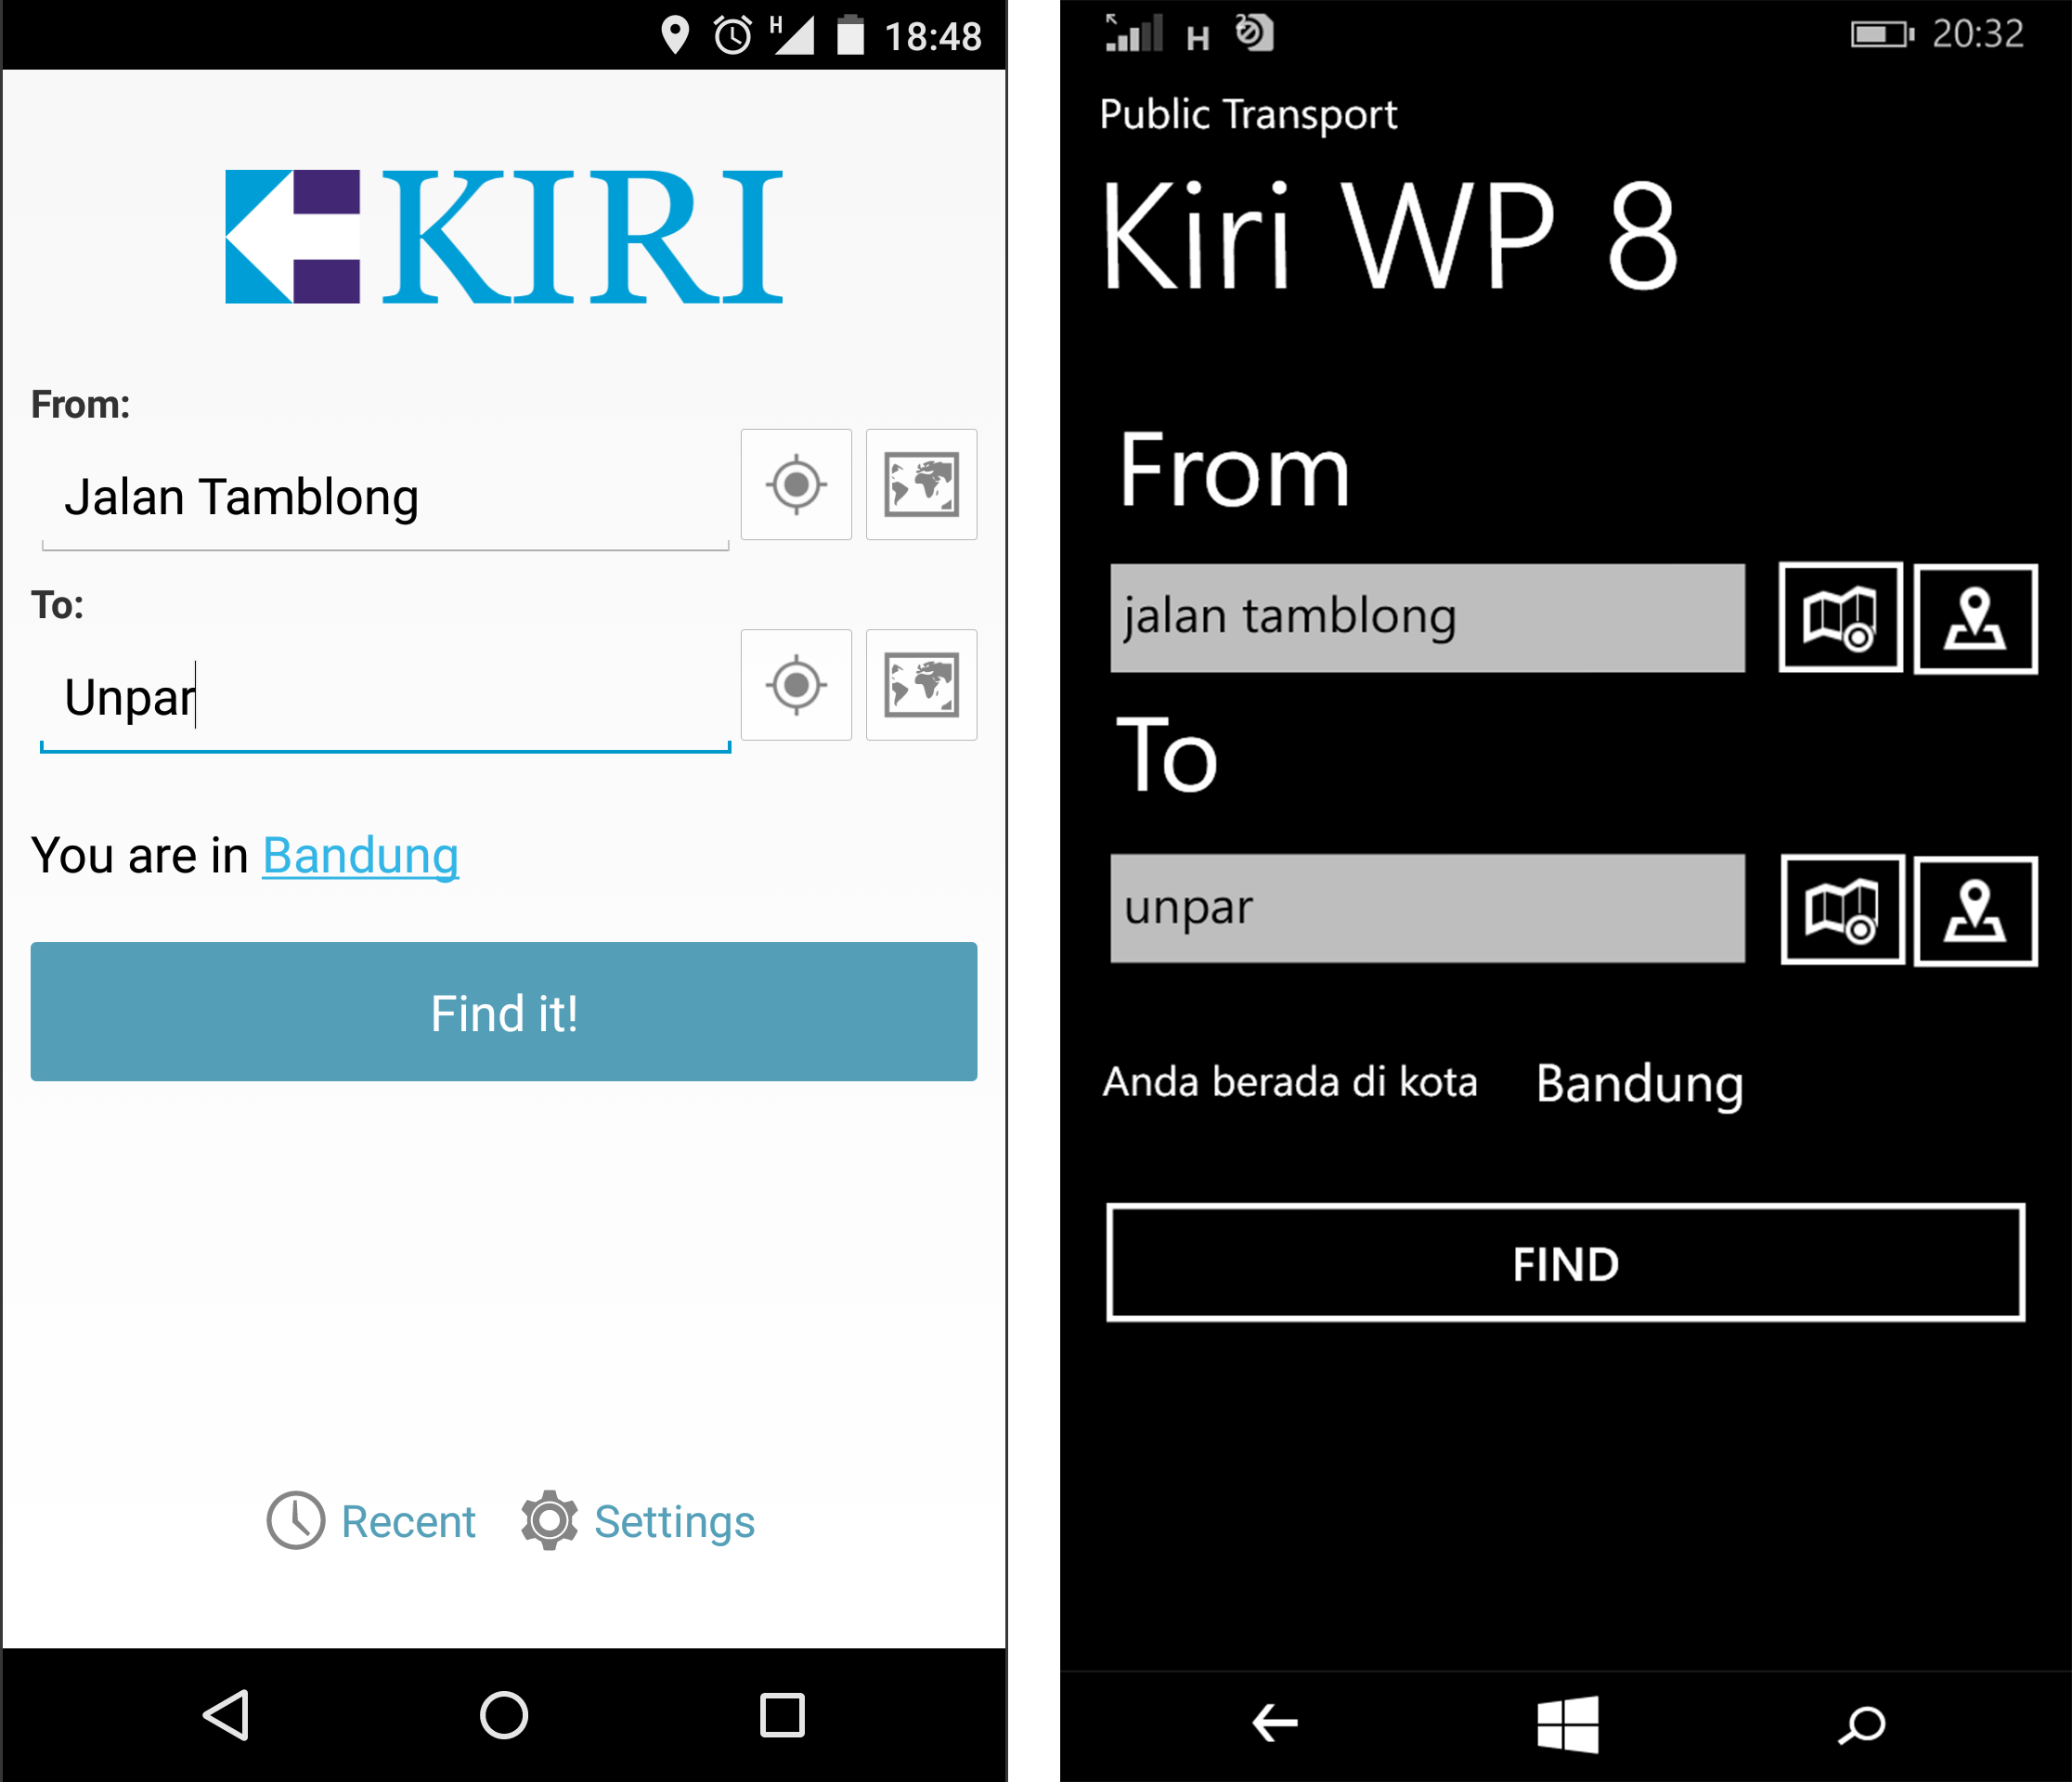
\includegraphics[scale=0.15]{Gambar/perbandingan/perbandingan_home}
%		\caption{Gambar Perbandingan Antarmuka \textit{Home} di Android(kiri) dan Windows Phone(kanan)}
%		\label{fig:perbandinganHome}
%	\end{figure}

% Gambar perbandingan home
%	\begin{figure}[!h]
%		\centering
%			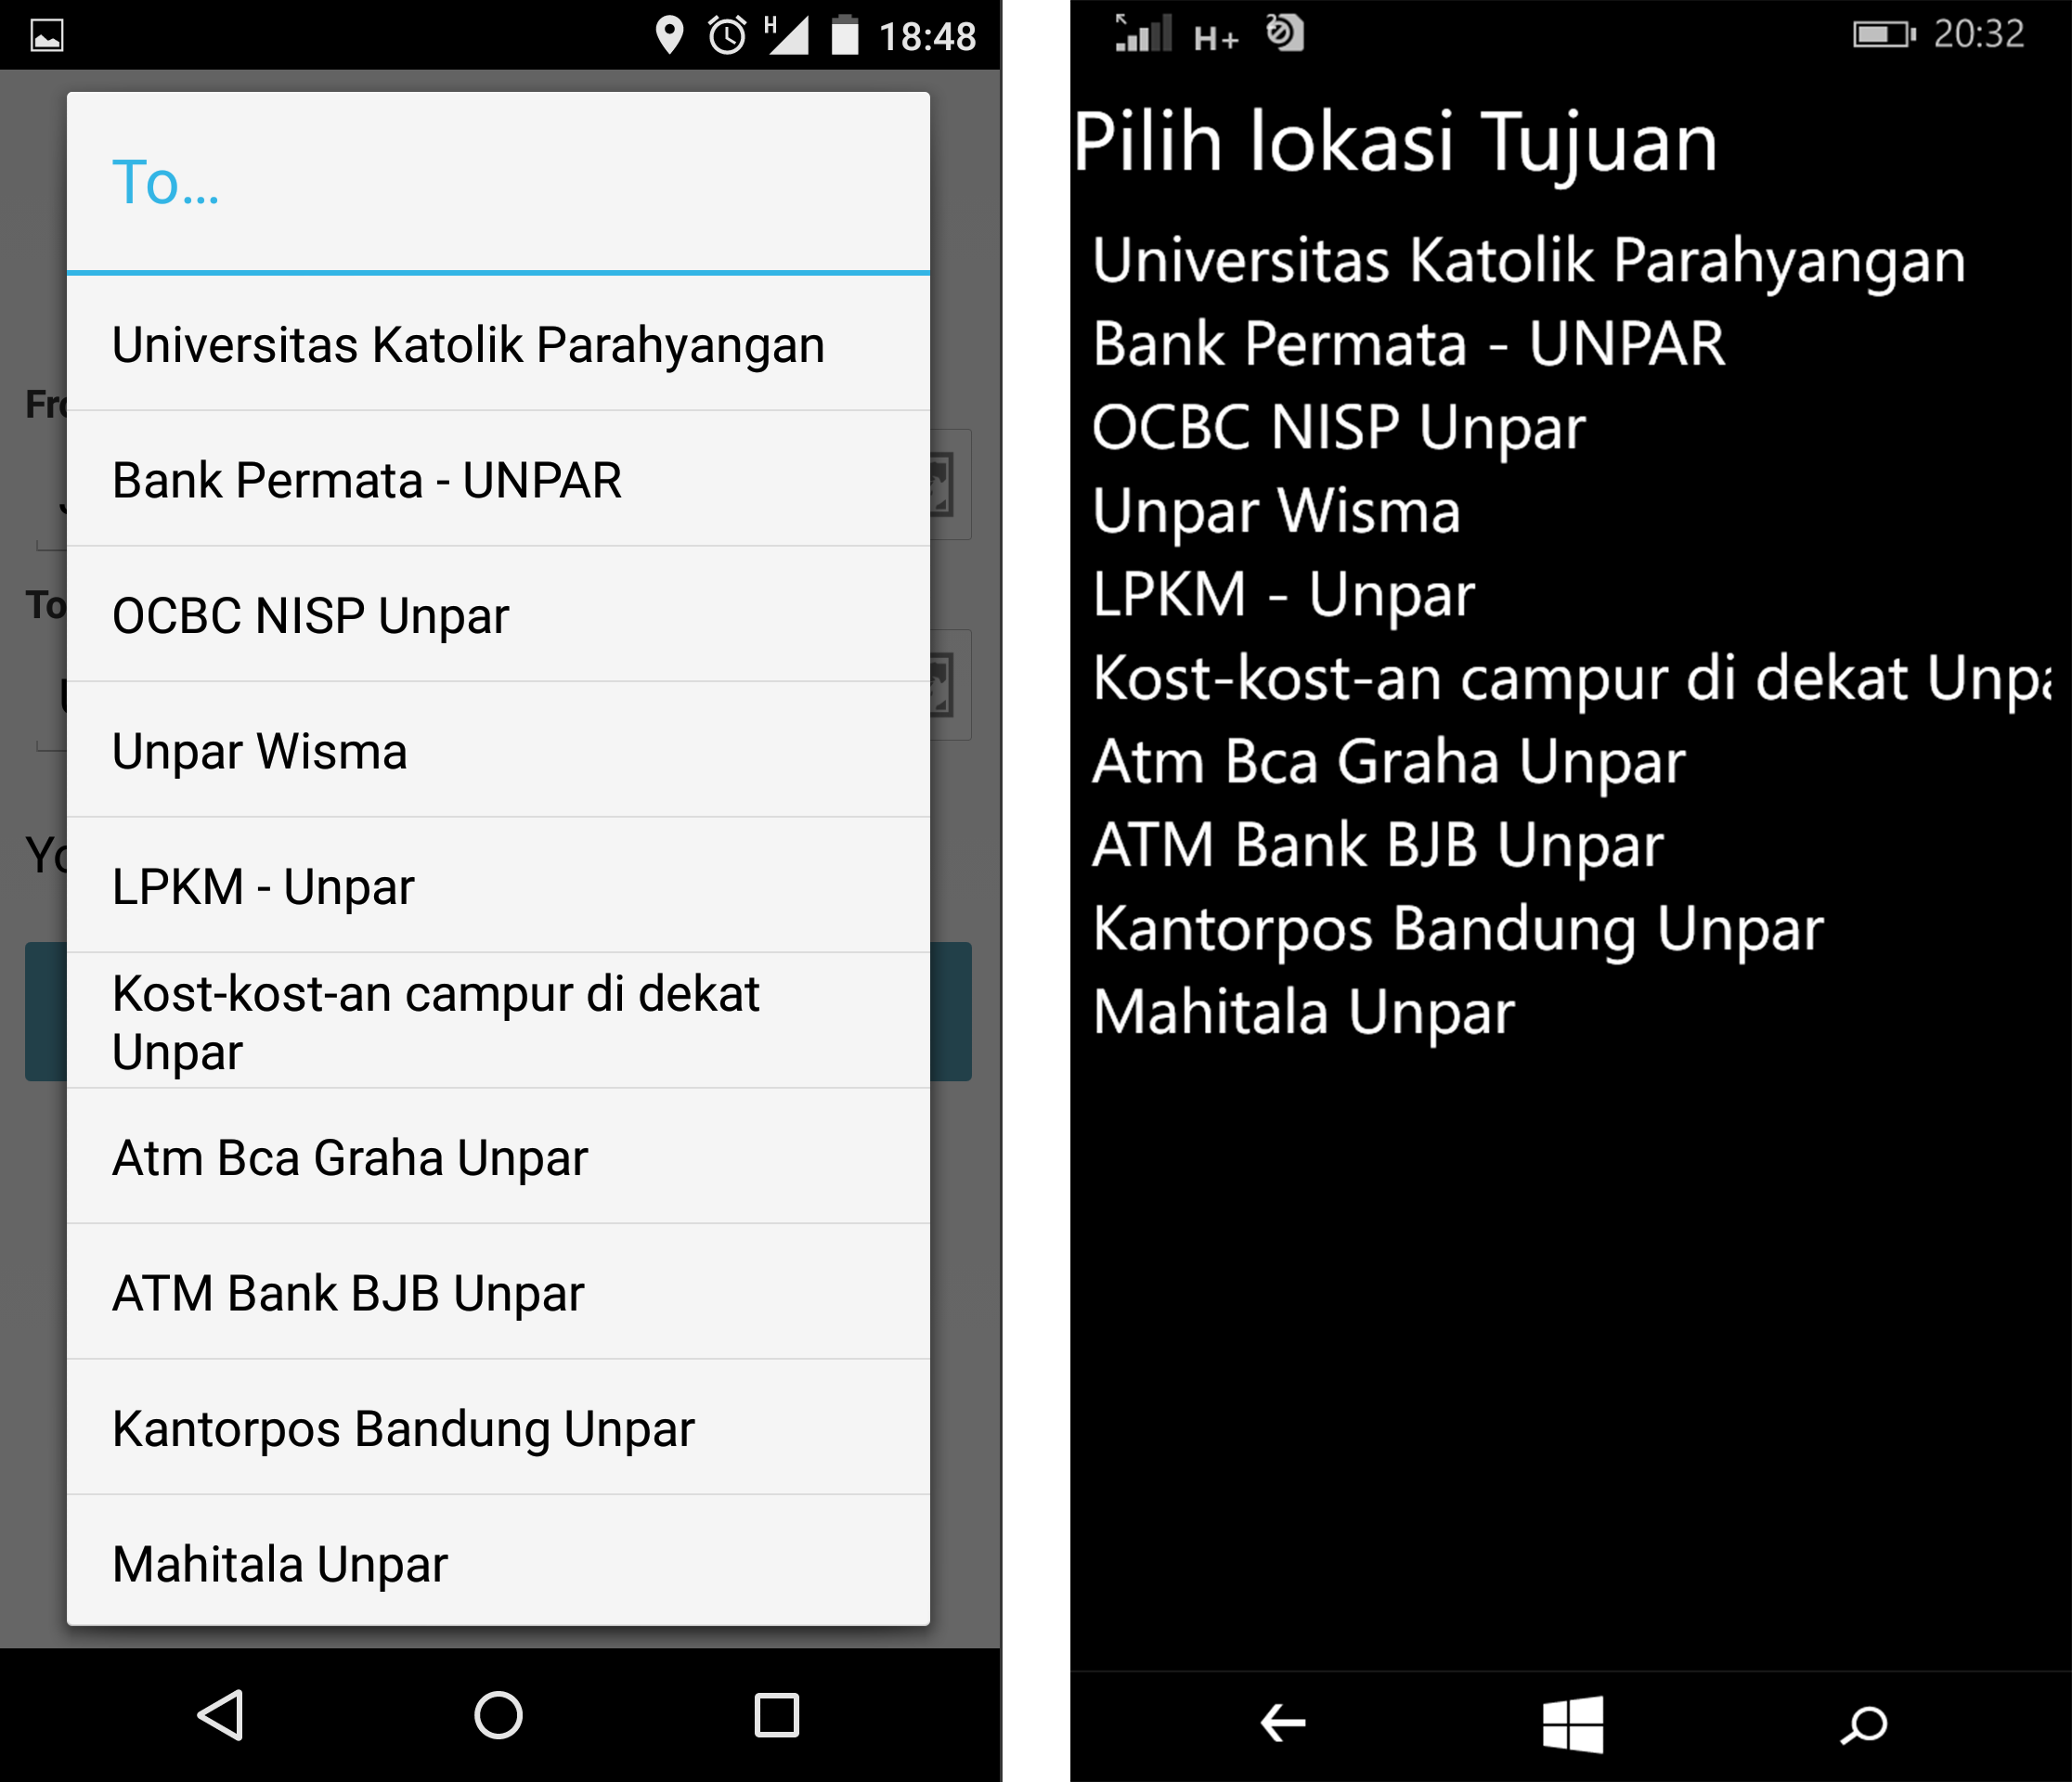
\includegraphics[scale=0.15]{Gambar/perbandingan/perbandingan_pilih}
%		\caption{Gambar Perbandingan Antarmuka Pemilihan Lokasi di Android(kiri) dan Windows Phone(kanan)}
%		\label{fig:perbandinganPilih}
%	\end{figure}
	
% Gambar perbandingan home
%	\begin{figure}[!h]
%		\centering
%			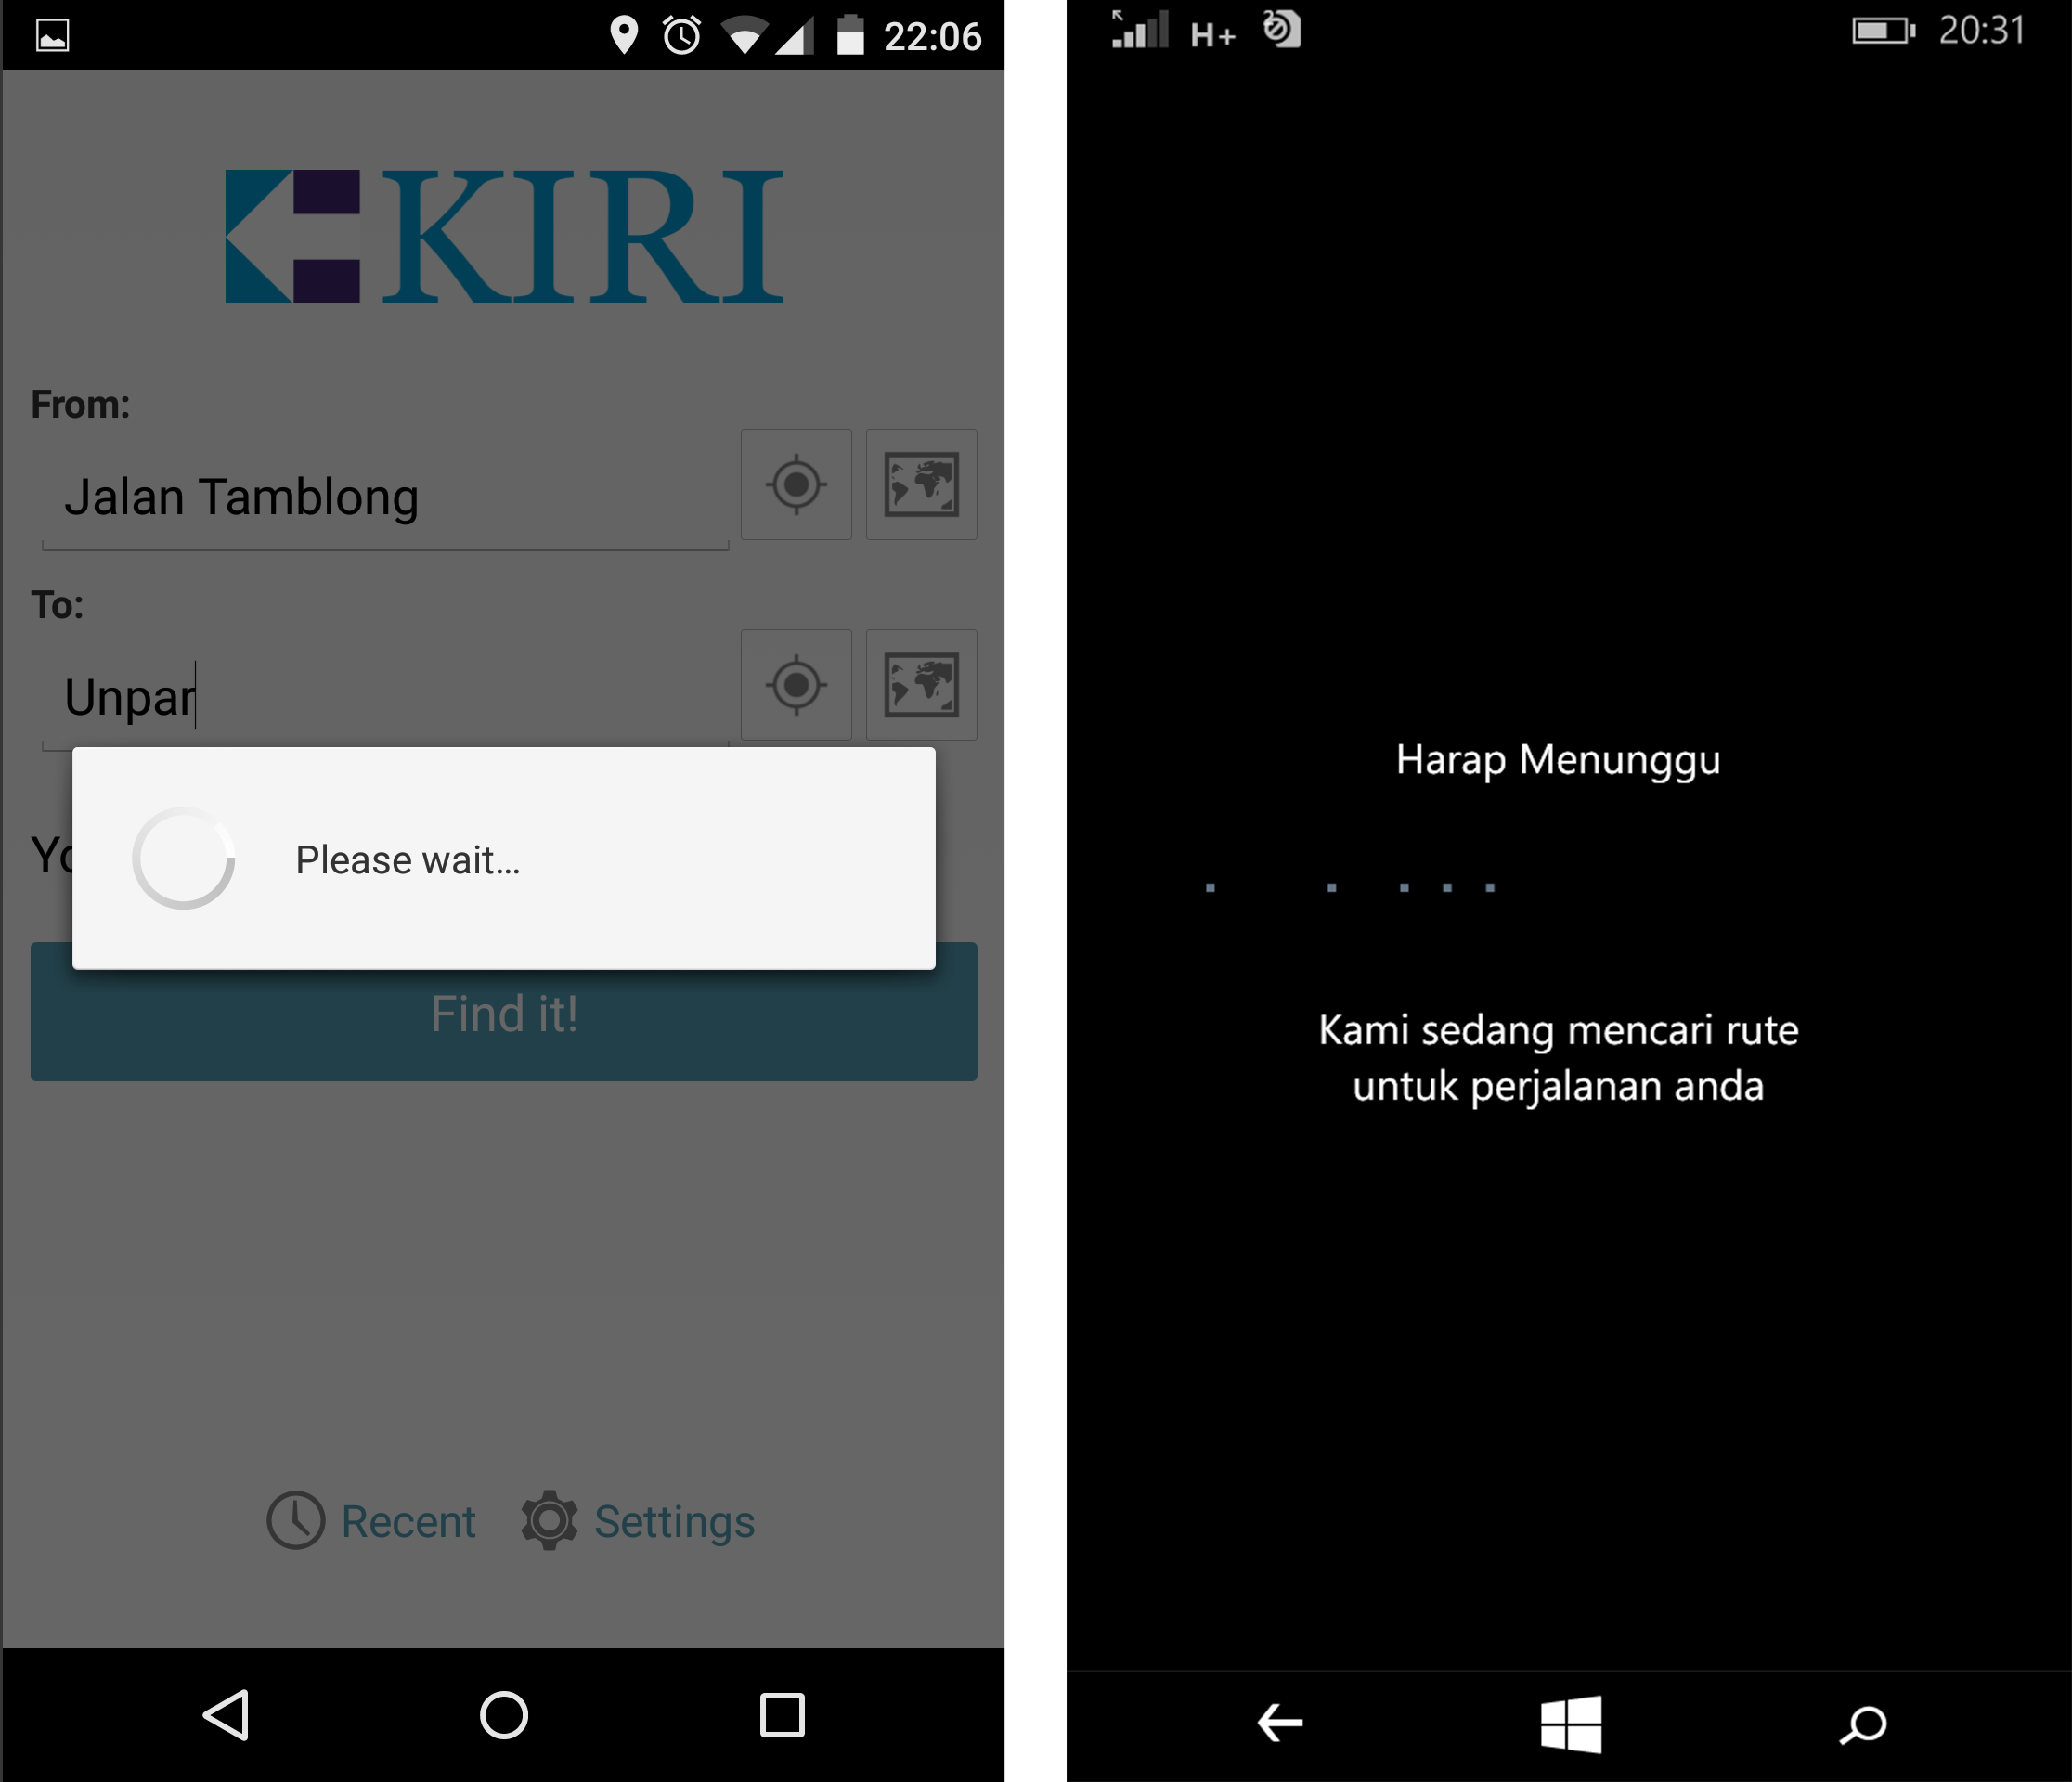
\includegraphics[scale=0.16]{Gambar/perbandingan/perbandingan_menunggu}
%		\caption{Gambar Perbandingan Antarmuka Menunggu hasil pencarian rute di Android(kiri) dan Windows Phone(kanan)}
%		\label{fig:perbandinganMenunggu}
%	\end{figure}
	
% Gambar perbandingan home
%	\begin{figure}[!h]
%		\centering
%			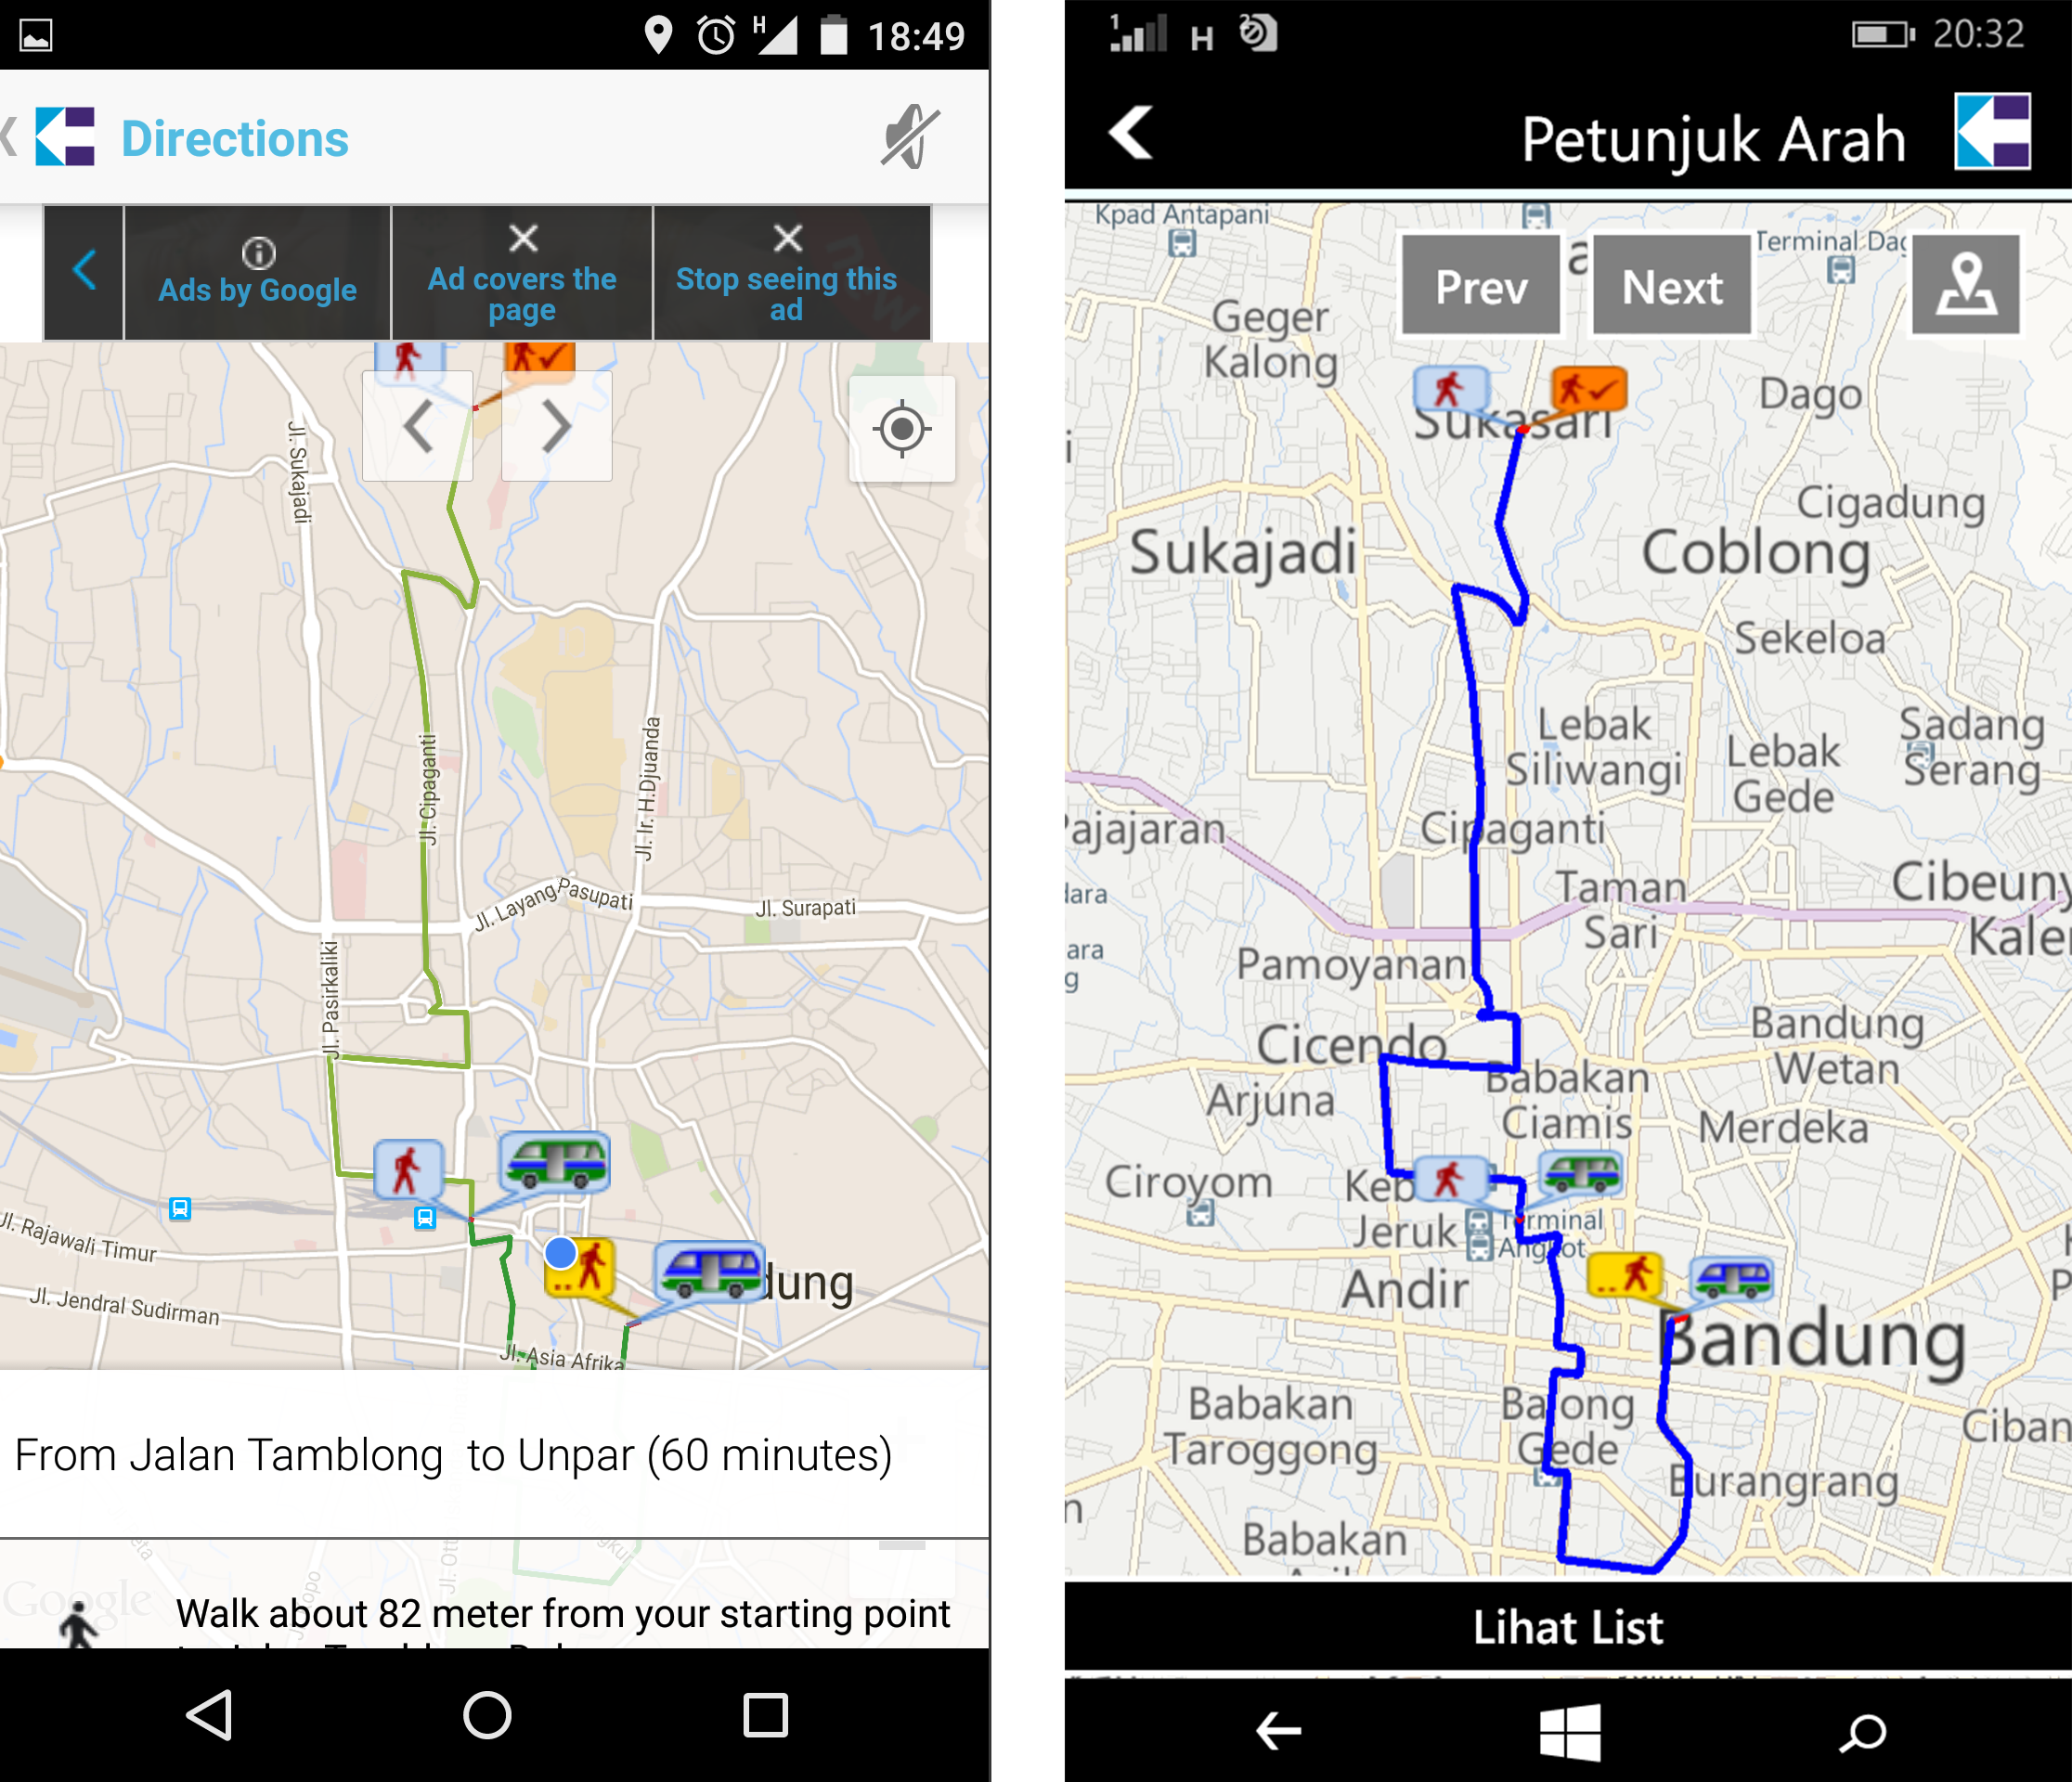
\includegraphics[scale=0.16]{Gambar/perbandingan/perbandingan_route}
%		\caption{Gambar Perbandingan Antarmuka Penentuan Rute di Android(kiri) dan Windows Phone(kanan)}
%		\label{fig:perbandinganRoute}
%	\end{figure}
	
%	\hspace{0.5cm} Dari hasil perbandingan aplikasi pencarian rute pada Android dan Windows Phone didapatkan kesimpulan sebagai berikut.
	
%	\begin{itemize}
%		\item Penunjuk lokasi perangkat menunjuk lokasi yang hampir sama ketika berada di ruangan terbuka.
%		\item Hasil penentuan lokasi dari kata kunci memiliki nilai yang sama.
%		\item Hasil penentuan rute sama-sama menunjukan keakuratan yang sama.
%	\end{itemize}

	
\subsection{Perbandingan Waktu pencarian Rute}
\label{lab:PerbandinganWaktu}
\hspace{0.5cm} Waktu menjadi hal yang penting bagi seseorang untuk menggunakan aplikasi. Pada pengujian ini dibandingkan waktu yang dibutuhkan dalam pencarian rute antara jaringan \textit{mobile} dengan Wi-Fi. Pengukur waktu dilakukan mulai dari aplikasi dibuka sampai rute berhasil didapatkan. Tempat pengujian dilakukan di rumah dan di Unpar. Berikut hasil perbandingannya.
   \begin{table}[h]
	\centering
		\begin{tabular}{|p{4cm}|p{4cm}|p{4cm}|}\hline
				Keadaan & Jaringan \textit{mobile} (detik) & Wi-Fi (detik) \\ \hline
				Dalam Rumah & 36 & 34\\ \hline
				Luar Rumah & 34 & 33\\ \hline
				Di Unpar & 37 & 35\\ \hline
				Rata-rata & 35.6 & 34\\ \hline
		\end{tabular}
	\caption{Tabel Perbedaan}
	\label{tab:TabelPerbandinganWifiSelular}
\end{table}

\hspace{0.5cm} Dari hasil pengujian didapat hasil bahwa hasil pencarian rute lebih cepat didapat jika menggunakan jaringan Wi-Fi. Hal tersebut dikarenakan kecepatan jaringan Wi-Fi lebih cepat dari pada jaringan \textit{mobile} yang menyebabkan data lebih cepat diterima perangkat. Hasil pengujian juga menunjukan hasil pencarian rute di dalam ruangan tertutup lebih lambat dari pada di luar ruangan. Pencarian rute di dalam ruangan yang lebih lambat dikarenakan GPS yang lebih lama mendapatkan lokasi dibandingkan jika perangkat berada di luar ruangan. 	
	
\subsection{Perbandingan Aplikasi Pencari Rute di Android dengan Aplikasi Pencari Rute di Windows Phone}
\label{lab:Perbandingan}
\hspace{0.5cm} Aplikasi Pencari rute yang dibuat dengan yang ada di Android memiliki beberapa perbedaan. Berikut perbedaan antara aplikasi pencari rute di Android dengan Windows Phone.

\begin{table}[h]
	\centering
		\begin{tabular}{|p{4cm}|p{4cm}|p{4cm}|}\hline
				Perbedaan & Android & Windows Phone \\ \hline
				Bahasa & Java dan antarmuka menggunakan XML & C\# dan antarmuka menggunakan XAML \\ \hline
				Mendapatkan Lokasi & Memanfaatkan pemanggilan lokasi secara berulang-ulang dan akan memperbarui lokasi dari yang kurang tepat menjadi lebih tepat. & Memanfaatkan pemanggilan sampai mendapat akurasi yang cukup tepat. \\ \hline
				Map  & Google Map & Windows Phone Map \\ \hline
				Navigasi antar halaman  & Pengiriman parameter berupa nilai "key" dan "value" & Pengiriman state objek \\ \hline
				Pemanfaatan sumber data & JSON in Java & Json.NET \\ \hline
		\end{tabular}
	\caption{Tabel Perbedaan}
	\label{tab:TabelPerbedaan}
\end{table}    